
\chapter{活动概念抽取}
\section{数据来源}
本文的工作基于新浪微博的数据。我们随机选取了100个用户作为种子,并获取他们的关注者和关注他们的人,以此为核心进行广度优先搜索。对每个用户,抓取其最近的1000条微博。表\ref{table:weibo_stat}是微博数据的一些信息:
\begin{table}[!h]
\centering
\begin{tabular}{|c|p{4cm}|}
\hline
用户数 & 1,787, 443 \\
\hline
微博数 & ~10亿 \\
\hline 
关注关系 & 40亿 \\
\hline 
用户信息 & 名字、性别、关注者,被关注者, 创建时间等 \\
\hline
微博信息 & 创建时间、评论数、转发数、原始微博、地理信息等 \\
\hline
\end{tabular}
\caption{微博数据概况}
\label{table:weibo_stat}
\end{table}

\section{候选集抽取}
\subsection{分词与词性标注}

由于中文没有天然的词边界,分词在处理中文语料是是基础的一步,也是重要的研究领域。常用的中文分词工具,如哈工大的LTP,中科院的ICTCLAS,Stanford Parser,实际应用中都难以做到非常高的准确度,尤其是在微博这种格式自由的文本中。综合比较各个工具的速度、精度后,我选择了ICTCLAS作为分词工具,同时对分出的词进行词性标注,并将常见的错误分词加入用户词典中提高分词精度。

\subsection{短语抽取}
依照我们对活动概念的定义\ref{def:concept},活动是单独的动词或一动宾结构的短语。为了挖掘出微博中表达的活动,我们需要将频繁出现的动词及短语抽取出来,以待进一步处理。

最简单的方法是,遍历语料,统计单独的动词,相邻的动词、名词的bigram的频度,按照词频保留TopK个。但这中简单的方法有一些问题
\begin{itemize}
\item 受停用词影响大。同英语语言一样,汉语中也存在一些停用词,如``是'',``在'', 在进行词性标注时被标注为动词,但并不表示一个实际动作。另一些虽然不是传统意义上的停用词,一般不做为一个动作,而是副词,如``完''”,``过'' 但经常出现在动词短语中,如``做完作业'',``吃过午饭''等。这些词常常词频很高,它们组成的短语数量多且排序高。
\item 表示活动的短语在文本中可能不是连续的。除了上面举过的例子之外,动词和名词之间可能包含一些更复杂的修饰成分,如``买了一件衣服'', ``参加学校举办的比赛''。对于这些情况,简单抽取相邻的动词、名词组成的bigram就会产生遗漏。
\item 倾向于选取包含高频词的短语,易受噪声影响。高频词会更多地和其他词随机共同出现,但并不构成一个短语。如果基于频度选取短语,会倾向于包含高频词的词组,无法将这种情况区分出来。
\end{itemize}

对于问题一,我们使用一个中文停用词词典,包含1220个停用词,对抽取结果进行过滤。对于问题二,我们的目标在于抽取常见的动词短语,而并不关注句法的精确解析,因此不需要很高的召回率,我们根据词性标签和词本身设计一些抽取规则,可以处理简单的包含数词、量词的情况。

对于问题三,一方面,一个短语应该出现足够多的次数,否则,它更有可能是随机噪声;另一方面,如果我们把词$w_i$是否出现作为随机变量$x_i$, 那么,如果$<w_i, w_j>$构成短语,那么$x_i$, $x_j$应该有比较强的相关性。相关性检验可以借助统计中的$\chi^2$检验。令$a=n(<w_i, w_j>), b=n(<w_i, \bar{w_j}), c=n(<\bar{w_i}, w_j), d=n(<\bar{w_i}, \bar{w_j}>), n=a+b+c+d$,如表\ref{table:chi}, $\chi^2$计算如下:
\begin{equation}
\chi^2 = \frac{n(ad-bc)^2}{(a+b)(c+d)(a+c)(b+d)}
\label{eqn:chi}
\end{equation}

\begin{table}
\centering
\begin{tabular}{|c|c|c|c|}
\hline
				& $w_j$ & $\bar{w_j}$	&	$sum$ \\
\hline
$w_i$ 			& $a$	& $b$ 			& $a+b$ \\
\hline
$\bar{w_i}$ 	& $c$	& $d$ 			& $c+d$ \\
\hline
$sum$ 			& $a+c$	& $b+d$ 		& $n=a+b+c+d$ \\
\hline
\end{tabular}
\caption{$\chi^2$检验}
\label{table:chi}
\end{table}

据此,可得到短语抽取算法\ref{alg:phrase_extraction}
\begin{algorithm}
\caption{Phrase Extraction}
\label{alg:phrase_extraction}
\KwIn{已分词的句集$S=\{s_i\}$,规则集合$R={r_i}$ $\lambda$, $K$}
\KwOut{短语集合$P = \{p_i\}$}

\ForEach {$s \in S$} {
    应用每条规则$r_i \in R$, 获得短语列表$P_{s}=[<w_i, w_j>]$。
    \ForEach {$p=<w_i,w_j> in P$} {
    	更新$n(<w_i, w_j>), n(w_i), n(w_j)$
    }
}

令$P_{raw}=\{<w_i, w_j>|n(w_i, w_j)>\lambda \}$\\

\ForEach {$p \in P$} {
	依照式\ref{eqn:chi}, 计算$\chi^2(p)$
}

以$\chi^2(p)$为键值,递减序排序$P$得到$P_{sorted}$\\

返回$P_{sorted}$的前$K$个元素
\end{algorithm}
最终,我们得到了90000条动词短语,作为活动概念的候选集。

\section{获取语义向量表示}
\label{sec:nnlm}
\subsection{背景和目标}
我们已经得到了一系列动词短语,作为活动的候选集合,但其中大多数并不表示一个日常活动,需要将活动概念加以区分。这是一个分类问题,可以使用现有的分类模型,关键在于特征的选取。

一种方法是,以词(unigram)作为特征。设共有$|V|$个不同的词,则bigram$<w_i, w_j>$的特征向量是一个$|V|$维向量$(0_1, 0_2,\ldots, 1_i, 0_i+1,\ldots, 1_j, 0_j+1, \ldots, 0_{|V|})$。这样做有效的原因是,动词和名词的数量是有限的,不同的短语可能包含相同的Action和Object,其中带有某些动词的短语,吃、喝,有更高的概率表示活动概念。如果我们进行足够的标注,覆盖足够多的情况,就可以对未知的短语进行分类。这种特征表示方法在计算语言学中称为One-hot Representation. 
但这样做的问题有
\begin{itemize}
\item 无法处理单个单词Unigram。One-hot Representation仅当不同短语间存在共同的单词才会有效。
\item 没有考虑不同词语的语义联系。假如两个词之间语义相似,那么他们的类标有更大的可能相同,而One-hot Representation中,不同单词是独立的。因此需要进行大量的标注,以覆盖尽可能多的样本。
\end{itemize}
在实际测试中,以SVM作为分类模型,可以达到82\%的分类精度,但召回率仅有29\%。为了避免大量的标注工作并提高召回率,我们需要寻找其他特征表示方法,以充分利用两个词之间的语义联系。

对语义相似度的计算,已经有许多方法。例如,基于文本片段中两个词的共现概率\cite{jiang1997semantic};基于搜索引擎查询结果条目数量\cite{bollegala2007measuring};将词表示为维基百科中条目的分布并计算余弦相似度\cite{liu2009clustering}。这些方法提供了两个词之间相似度的度量,但使用并不方便。理想的情况是将每个词表示为$K$维空间的向量,K远远小于不同词的总数,词之间的相似度可以计算两个向量的余弦相似度。这Hinton提出的Distributed Representation\cite{hinton1986learning}。本文使用基于神经网络语言模型的工具Word2Vec获得词语的语义向量表示。

\subsection{神经网络语言模型(NNLM)}
要对语义进行建模,容易想到的思路是,假如两个词经常出现的上下文相似,那么它们的语义可能也是相似的,这是自然语言处理中了统计语言模型的基础。一个语言模型是语言基本单位(如句子)的生成模型,用各个单词出现的条件概率来表示,即
\[
p(sentence) = \prod\limits_t {p({w_t}|Context_t)}
\]
Context的选取不同,语言模型也随之变化,其中n-gram语言模型是其中常用的一种。它对语言的生成做了n-1阶Markov假设,一个词的出现概率仅和前n-1个词相关,即
\begin{align*}
Context_t = & w_{t-n+1}^{t-1} \\
		= & (w_{t-n+1}, w_{t-n+2}, \ldots, w_{t-1}) \\
p(sentence) = & \prod\limits_t {p({w_t}|w_{t-n+1}^{t-1})}
\end{align*}

n-gram语言模型的问题是,由于语料的限制,高阶的语言模型受制于数据的稀疏性,无法建模更远的关系,一般使用tri-gram。随着互联网带来的海量数据以及计算能力的提升,更高阶的语言模型成为可能,Google曾经公开了5-gram的语言模型,但体积非常大,对我们的应用来说不切实际的。其次,n-gram对语义相似度建模的能力有限。它仅考虑词在给定上下文出现的概率,但对上下文的相似性没有考虑。比如,``房间里趴着一只狗''和``卧室里趴着一只猫'',对``猫''和``狗''建模时,n-gram模型没有考虑``房间''和``卧室''的相似性,而它们的相似性是可以根据其他文本得到的。我们需要找到一种可以将上下文相似性一并考虑的方法模型。

换个角度思考,我们要求的是$p({w_t}|w_{t-n+1}^{t-1})$, 实际可以看做是一个函数$f(w_{t-n+1}, w_{t-n+2}, \ldots, w_{t-1}, w_t)$. Hornik等人证明了,带有一个隐含层的多层前馈神经网络,可以近似$R^n$上任意连续函数(universal approximation theorem\cite{hornik1991approximation}). 因此,我们也能用神经网络来逼近$f()$. 我们把$w_{t-n+1}, w_{t-n+2}, \ldots, w_{t-1}$的One-hot Representation作为输入,希望输出$output_i=P(w_t=i|w_{t-n+1}, w_{t-n+2}, \ldots, w_{t-1})$, 这样就是n-gram语言模型的神经网络近似。如果我们把输入换成每个词对应的K维向量表示,那么上下文的相似性可以自然体现在向量的相似性中,这个模型就是神经网络语言模型(NNLM)\cite{bengio2006neural} \cite{mikolov2013efficient}。与一般神经网络不同的是,它的输入,即每个词的向量表示,是未知的,需要和模型参数一同优化。如图\ref{fig:nnlm}所示,输入为词序列$w_{t-n+1}^{t-1}$,$C(w_i)$为词$w_i$的向量表示,输出经过softmax归一化为词出现的概率。可用随机梯度优化网络参数。由于输出层为softmax,不会出现概率为0的情况,因此不需n-gram模型中复杂的平滑方法,并且可以取得更好的效果。

\begin{align*}
y = & b+U\tanh(d+Hx)\\
output_t = & P(w_t|w_{t-n+1}^{t-1}) \\
		= & \frac{e^{y_i}}{\sum\nolimits_i {{e^{{y_i}}}} }
\end{align*}

\begin{figure}[htbp]
\centering
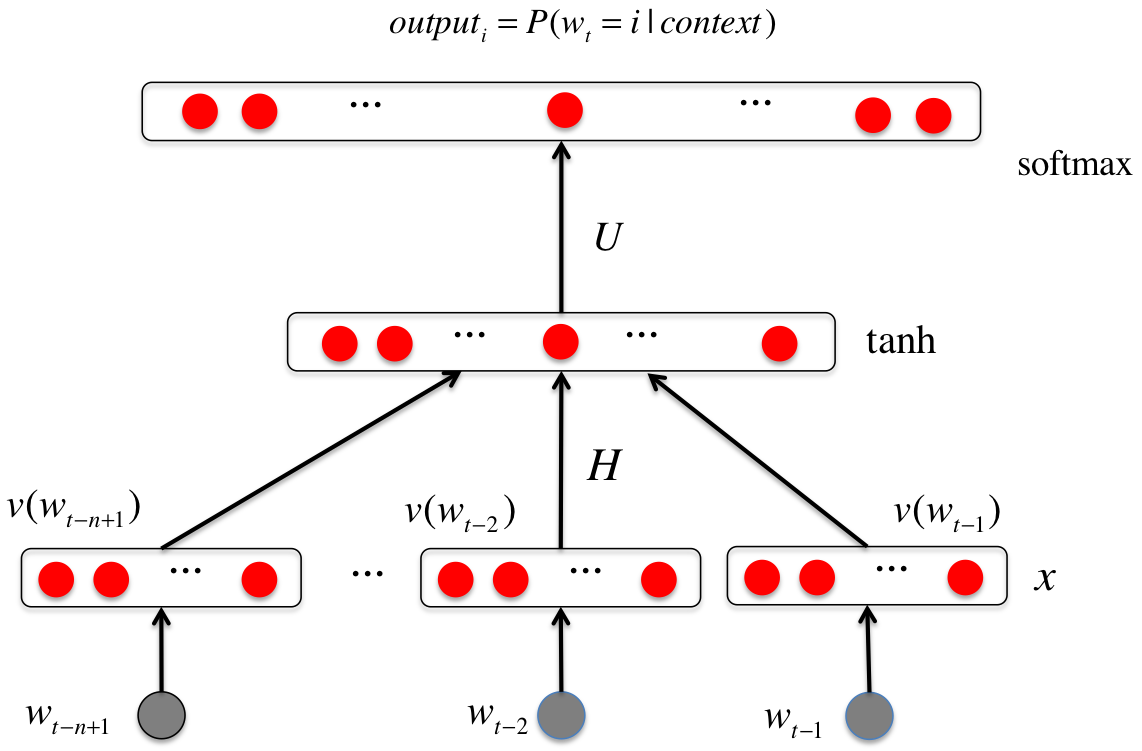
\includegraphics[width=0.8\textwidth]{nnlm.png}
\caption{神经网络语言模型}
\label{fig:nnlm}
\end{figure}

Google Word2Vec提供了使用前馈神经网络对神经网络语言模型进行训练的高效工具。

\subsection{案例研究}
我们在1300万条新浪微博上训练了NNLM,并对得到的向量做一些案例研究,以检验模型的有效性。

首先,我们给出一个活动,用余弦相似度衡量两个词语义上的相关性,找出和其最相似的10个词组,如表\ref{table:similarity_instances}。可见,根据NNLM得到的向量表示,很好地反映了语义的相似性。

\begin{table}[h]
\centering
\begin{subtable}{0.3\textwidth}
     \begin{tabular}{|l|c|} 
	\hline
	{\heiti 短语} & {\heiti 相似度} \\
	\hline
	打\_篮球 & - \\
	\hline
	打球 & 0.800 \\
	\hline
	踢\_足球 & 0.790 \\
	\hline
	打\_网球 & 0.789 \\
	\hline
	打\_羽毛球 & 0.797 \\
	\hline
	踢球 & 0.727 \\
	\hline
	踢\_球 & 0.697 \\
	\hline
	练\_球 & 0.686  \\
	\hline
	游泳 & 0.667 \\
	\hline
	排球 & 0.651 \\
	\hline
	打\_排球 & 0.649 \\
	\hline
	\end{tabular}
\end{subtable}
\hspace{1em}
\begin{subtable}{0.3\textwidth}
	\begin{tabular}{|l|c|} 
	\hline
	{\heiti 短语} & {\heiti 相似度} \\
	\hline
	打扫 & - \\
	\hline
	打扫\_卫生 & 0.805 \\
	\hline
	收拾 & 0.757 \\
	\hline
	洗\_衣服 & 0.747 \\
	\hline
	家里\_打扫 & 0.699 \\
	\hline
	收拾\_屋子 & 0.693 \\
	\hline
	搞\_卫生 & 0.666 \\
	\hline
	捣鼓 & 0.659 \\
	\hline
	打扫\_打扫 & 0.659 \\
	\hline
	洗\_床单 & 0.654 \\
	\hline
	拖\_地板 & 0.652 \\
	\hline
	\end{tabular}
\end{subtable}

\begin{subtable}{0.3\textwidth}
	\begin{tabular}{|l|c|} 
	\hline
	{\heiti 短语} & {\heiti 相似度} \\
	\hline
	吃\_晚饭 & - \\
	\hline
	吃\_午饭 & 0.920 \\
	\hline
	晚饭 & 0.844 \\
	\hline
	吃\_中饭 & 0.831 \\
	\hline
	吃饭 & 0.816 \\
	\hline
	吃\_夜宵 & 0.795 \\
	\hline
	吃\_早饭 & 0.780 \\
	\hline
	午饭 & 0.777 \\
	\hline
	出去\_觅食 & 0.755 \\
	\hline
	中午\_饭 & 0.746 \\
	\hline
	喝\_早茶 & 0.736 \\
	\hline
	\end{tabular}
\end{subtable}
\hspace{1em}
\begin{subtable}{0.3\textwidth}
	\begin{tabular}{|l|c|} 
	\hline
	{\heiti 短语} & {\heiti 相似度} \\
	\hline
	下班 & - \\
	\hline
	上班 & 0.751 \\
	\hline
	回家 & 0.748 \\
	\hline
	下班\_回家 & 0.730 \\
	\hline
	坐\_班车 & 0.716 \\
	\hline
	提早\_下班 & 0.706 \\
	\hline
	回到\_家 & 0.705 \\
	\hline
	十一点\_半 & 0.705 \\
	\hline
	五点\_下班 & 0.703 \\
	\hline
	吃\_晚饭 & 0.701 \\
	\hline
	收工 & 0.698 \\
	\hline
	\end{tabular}
\end{subtable}

\caption{语义相似度实例}
\label{table:similarity_instance}
\end{table}

并且词向量具有可加性.例如, 可以用向量加法来表达语义关系的组合:
\begin{align*}
	v(\text{济南}) - v(\text{山东}) + v(\text{浙江}) \rightarrow & v(\text{杭州}) \\
	v(\text{北京}) - v(\text{中国}) + v(\text{法国}) \rightarrow & v(\text{巴黎}) \\
\end{align*}
这里的$\rightarrow$表示,在所有的词中,约等号右边的词向量与左边运算的结果余弦相似度最大.这两个式子的含义是,杭州对浙江的关系,与济南对山东的关系相似(都是省会); 东京对日本的关系,与北京对中国的关系相似(都是首都).

再如
\begin{align*}
	v(\text{喝}) - v(\text{渴}) + v(\text{饿}) \rightarrow & v(\text{吃}) \\
	v(\text{校长}) - v(\text{学校}) + v(\text{公司}) \rightarrow & v(\text{总裁}) \\
	v(\text{胡锦涛}) - v(\text{中国}) + v(\text{日本}) \rightarrow & v(\text{首相}) \\
\end{align*}
这些式子都有很明确自然的语义关系。虽然这种语义组合的关系并不是总能成立,但反映出,词的向量表示在某种层面上反映了词的语义特征。

\section{最优化标注集}
\subsection{目标}
在\ref{sec:nnlm}中,我们得到了每个词对应的向量表示。对于unigram, 词向量本身就是短语的向量;对于bigram, 由于向量可加,将动词和名词的向量相加后归一化,如此,每个动词短语可以看做K维语义向量空间中的一个向量,更确切来说,每个向量的模长均为1,它们分布在一个K维超球面上。

在对短语进行分类前,需要手工构建一个标注集,类标``1''表示是活动,``0''表示非活动,作为训练数据训练分类模型,确定模型参数。传统上,训练样本是从待分类数据中随机抽样得到。由于语义空间很大,待分类的数据也比较多,使用随机抽样得到的训练样本训练SVM分类器,精度为69\%, 召回率相对One-hot Representation有所提升,但依然只有43\%。更多的标注可以改善精度和召回率的情况,但大量标注需要耗费很常时间。本文希望根据数据分布的特性,希望设计一种有原则的训练样本选择方法,在标注数据量一定的情况下,能够尽可能提高训练的效果。假设标注集为$L$,我们需要恰当定义其效用函数$Q(L)$以判断它的有效性,并且限制$L$的大小为$M$,找出最优的$L$,也就是
\[
    L^* = \arg\max_{L,|L| = M} Q(L)
\]

\subsection{模型概述}
直觉上,标注一个训练样本后,和此训练样本相似的样本,我们有较高的置信度将其正确分类。例如,在K近邻分类器中,对于每个未知样本,寻找训练集中和其距离最近的K个样本,由这K个近邻投票确定此样本的类标; 在SVM中,若$x_i \sim x_j$,则$wx_i+b \sim wx_j+b$。

在我们的问题中,样本间的相似性$sim(x_i, x_j)$使用向量的余弦相似度来表示$<x_i, x_j>=\frac{x_i\dot x_j}{|x_i||x_j|}$,据此可以定义一个样本$x$和集合$S$的相似性。

\begin{definition}
\[
    sim(x, S) = \mathop {\max }\limits_{u \in S} sim(x,u)
\]
\end{definition}
即,样本$x$与集合$S$的相似度为$S$中与$x$最相似的元素与$x$的相似度。

设全部数据样本的集合为$U$, 标注集为$L$, 我们希望对于每个未知样本,在$L$中,都能找到一个与其相似度高的的元素,即标注集能够更好地代表所有数据。根据这个想法,我们的效用函数可以定义成
\[
    Q(L) = \mathop {\min }\limits_{{v_i}} sim({v_i},L)
\]
意义是,所有样本与$L$的最小相似度。$Q(L)$越大,说明$L$越好地代表了数据集。我们的目标是,限制$L$的大小为$M$,找到最优的标注集$L^*$。问题可以形式定义为:

\begin{problem}\label{prob:opt_problem}
给定集合$U$, 对任意元素$x_i, x_j \in U$, 有相似度度量$sim(x_i,x_j)$. 元素与集合相似度$sim(x, S)$和效用函数$Q$如前定义。要求最优子集
\[
        {L^*} = \mathop {\arg \max }\limits_{L \subseteq U, \ |L| = M} Q(L)
\]
\end{problem}

\subsection{NP-Hardness}
\label{sec:nph}
问题\ref{prob:opt_problem}是一个组合优化问题,这类问题通常是NP-Hard的,下面我们将集合覆盖问题可以归约到此问题来证明其NP-Hardness。

集合覆盖问题的判定版本是Richard Karp在1971年提出的21个NP完全问题之一。问题定义为:

\begin{problem}[集合覆盖]
\label{prob:set_cover}
给定全集$U$,一族子集$S=\{S_i\}, \cup {S_i} = U$,以及整数$M$,判定是否存在覆盖$[C \subseteq S,|C|=M$,使得$\cup \{ {S_i}|{S_i} \in C\}  = U$
\end{problem}

问题\ref{prob:opt_problem}的判定问题是
\begin{problem}[问题\ref{prob:opt_problem}的判定问题]
\label{prob:dec_problem}
给定阈值$\theta$,判定是否存在大小为$M$的集合$L$,使得
\[
    \theta  \le \mathop {\min }\limits_{{x_i} \in U} \mathop {\max }\limits_{{x_j} \in L} \{ sim({x_i},{x_j})\} 
\]
\end{problem}

如果能证明此判定问题的NP完全性,那么原问题的NP-Hardness就得证。显然,如果能解决集合覆盖问题,问题\ref{prob:dec_problem}也可得到解决。但为了证明\ref{prob:dec_problem}的NP完全性,需要进行相反方向的归约,即证明,如果能在多项式时间解决问题\ref{prob:dec_problem}, 则集合覆盖问题也可在多项式时间解决。证明如下。

\begin{proof}
对于集合覆盖问题\ref{prob:set_cover},如果存在一个元素$x \in U$不在任何一个$S_i \in S$中,那么覆盖显然是不存在的.下面仅考虑每个元素都至少被一个$S_i \in S$覆盖的情况。

设$|U| = N, |S| = P$, 我们构造一个包含$N+P$个结点的图$G=(V,E)$。其中,结点集$V$为:
\begin{itemize}
\item 集合$U$中的每个元素$x_i, 1 \le i \le N $ 都对应$G$中的一个结点$v_i$,称为元素结点(element nodes)。
\item 对每个$S_i \in S$, 对应节点$v_{i+N}, 1 \le i \le P$, 称作集合结点(set nodes)。
\end{itemize}
边集$E=\{(v_i, v_{j+N}) | v_i \in S_j, 1\le i \le N, 1\le j \le P\} \cup {(v_i+N, v_j+N) | 1 \le i,j \le P}$. 即,每个集合都和它包含的元素连边,集合之间两两连边。所有边赋权为$\theta$,不存在边的赋权负无穷。如图\ref{fig:setcover}所示。
\begin{figure}[htbp]
\centering
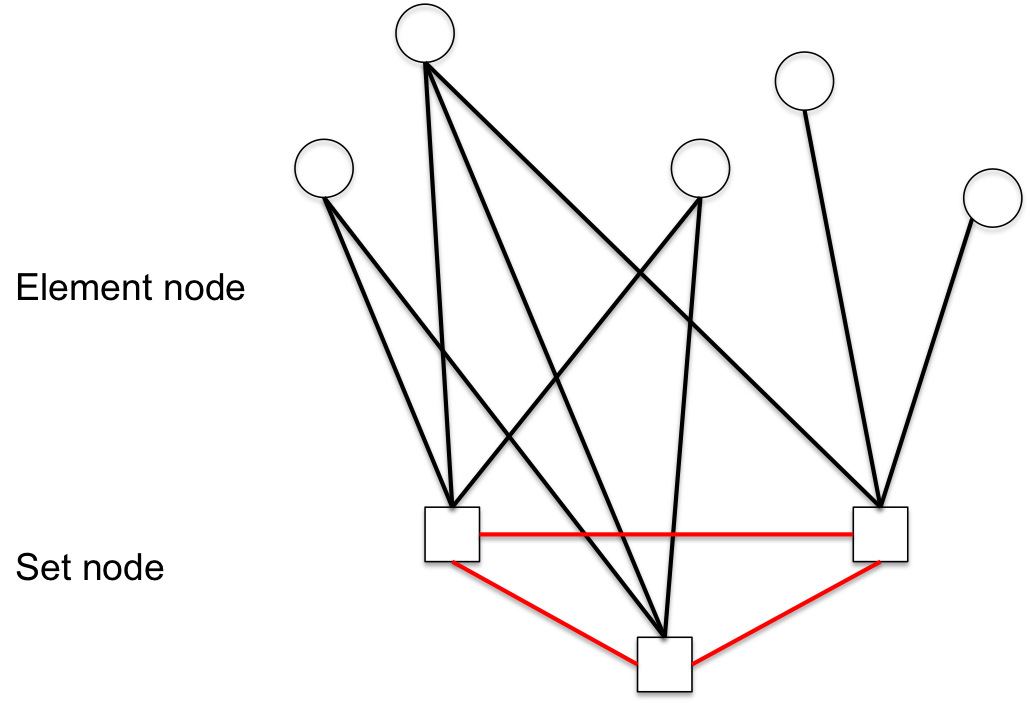
\includegraphics[width=0.7\textwidth]{./setcover.png}
\caption{问题归约}
\label{fig:setcover}
\end{figure}

假如我们能在多项式时间内求解问题\ref{prob:dec_problem}, 则分两种情况。

1, 如果存在满足条件$L$,可在多项式时间构造集合覆盖问题的解$C$:对任意$v_i \in L$, 若$v_i$为集合结点(即$N+1 \le i \le N+P$),则$S_i \in C$;若$v_i$为元素结点($N+1 \le i \le N+P$), 取任意包含$v_i$的任意集合$x_i \in S_j$,使得$S_j \in C$。这样,$C$构成了$U$的一个覆盖。

2, 如果$L$不存在,则集合覆盖也不存在。否则,若存在$U$的一个覆盖$C$, 选择$C$中集合对应的结点构成$L$,就可以得到问题\ref{prob:dec_problem}的解,矛盾。

这样,集合覆盖问题就在多项式时间内归约到了问题\ref{prob:dec_problem}。又由于它也可以归约到集合覆盖问题,因此,问题\ref{prob:dec_problem}是一个NP完全问题。其优化版本,即我们要求解的问题\ref{prob:opt_problem},是一个NP-Hard问题。不存在已知的多项式时间解。
\end{proof}

\subsection{子模性及近似求解}

节\ref{sec:nph}已经证明最优化$Q(L)$是一个NP-Hard问题,但是下面我们将证明其单调性和子模性,并据此得到一个贪心算法(greedy algorithm), 在多项式时间内得到近似解$Q(L')$, 并且保证
\[
	Q(L') \ge (1-\frac{1}{e}) Q(L^*)
\]

首先给出子模函数(submodular function)的定义。
\begin{definition}[子模函数]
从幂集$2^\Omega \to R$的一个函数$f$称为子模函数,如果对任意$X,Y \subseteq \Omega, X \subseteq Y$,$\forall x \notin Y$, 有$f(X \cup \{x\} ) - f(X) \geq f(Y \cup \{x\} ) - f(Y)$.
\end{definition}

下面我们分别证明$Q(L)$的单调性和子模性。单调性是显然的。
\begin{proof}[单调性]
令集合$Y=X\cup{x}$。对任意元素$y \in U$, 设$sim(y, X) = sim(y, t), t \in X$, 即对任意$x \in X$, $sim(y,x) \le sim(y,t)$。

由于$X \subset Y$,故有
\begin{align*}
	sim(y,Y) = & \mathop {\max }\limits_{x \in Y} sim(y,x) \\
			\ge &  \mathop {\max }\limits_{x \in X} sim(y,x) \\
			\ge &  sim(y,X) \\
\end{align*}
从而, $sim(y, Y) \ge sim(y, X)$。由$y$的任意性,得到

\begin{align*}
	Q(Y) = & \mathop {\min }\limits_{y \in U} sim(y,Y) \\ 
		\ge & Q(X)
\end{align*}

单调性证完。
\end{proof}

\begin{proof}[子模性]
设集合$X \subset Y$, 对任意$x \in U - Y$, 设$X' = X\cup{x}, Y' = Y\cup{x}$。对任意$y \in U$, 由单调性有
\begin{eqnarray*}
	sim(y, Y') \ge sim(y, X') \ge sim(y, X) \\
	sim(y, Y') \ge sim(y, Y) \ge sim(y, X) 
\end{eqnarray*}

对于新加入的元素$x$, 有
\begin{align*}
	sim(y, X') = & \max\{ sim(y, x), sim(y,X) \} \\
	sim(y, Y') = & \max\{ sim(y, x), sim(y,Y) \} \\
\end{align*}

于是
\begin{align*}
	sim(y, Y') - sim(y, Y) = & \max \{ sim(y, x) - sim(y, Y), 0\} \\
						\le & \max \{ sim(y, x) - sim(y, X), 0 \} \\
						= & \max \{ sim(y, x), sim(y, X) \} - sim(y, X) \\
						= & sim(y, X') - sim(y, X)						
\end{align*}
由$y$的任意性,子模性得证。
\end{proof}

对于单调非减的子模函数,有以下定理
\begin{theorem}
对于一个单调增的子模函数$Q$,从空集$L_0$开始,使用贪心策略进行迭代,即第$k$次迭代选取元素$v_k$,使得
\[
	v_k = \mathop {\arg \max }\limits_{v_k \notin L_{k-1} } Q(L_{k-1}\cup \{v_k\}) 
\]
\[
	L_k = L_{k-1} \cup \{ v_k \} 
\]
那么$K$次迭代之后, 对任意$L, |L| \le K$,有
\[
	Q(L_k) \ge (1-\frac{1}{e}) Q(L),
\]
\end{theorem}

这直接给我们了一个保证下界的贪心算法。
\begin{algorithm}
  \caption{maximize Q(L)}
  \KwIn{Unisersal set $U$, target size $K$ and similarity measure $sim()$}
  \KwOut{${L^*} = \mathop {\arg \max }\limits_{L,|L| = K, L \subseteq U} Q(L)$ }
  $L_0 = \emptyset$\;
  \For{$k=1;k \le K;k += 1$}
  {

  }
  return $con(r_i)$\;
\end{algorithm}

\section{模型选择}
我们的标注集选择和KNN有密切的联系,KNN在我们的数据中可能表现更好,但是我们也会尝试其他的分类模型,如支持向量机,随机森林等。

\section{实验结果与错误分析}
为了检验我们标注和分类的效果,我们从短语候选集中随机抽取了5000个短语作为Ground Truth进行测试。

图\ref{fig:testing_vs_random}是我们分别使用随机抽样(Random)和最大化$Q(L)$(MaxSim)的方法选取500、1000、2000个标注样本时,5-NN分类器在测试集上的表现。对于随机抽样,我们进行5次试验取平均值,并在图中标注了最大和最小值。

\begin{figure}[h!]
  \centering
  \begin{subfigure}{0.4\textwidth}
    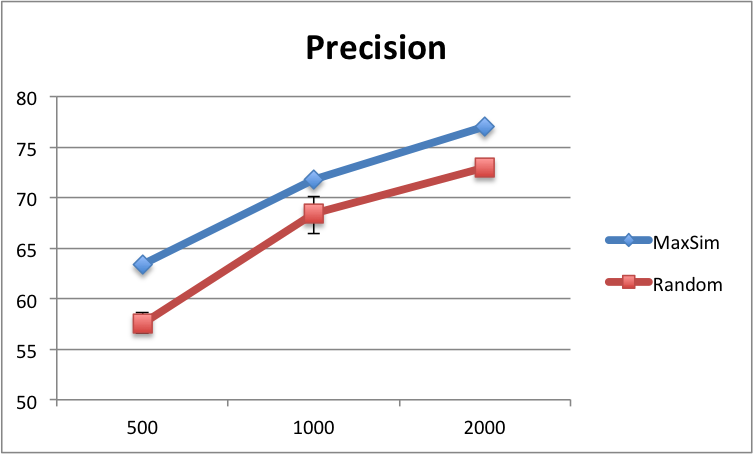
\includegraphics[width=\textwidth]{label_precision.png}
    \caption{Precision}
  \end{subfigure}
  \hspace{2em}%
  \begin{subfigure}{0.4\textwidth}
    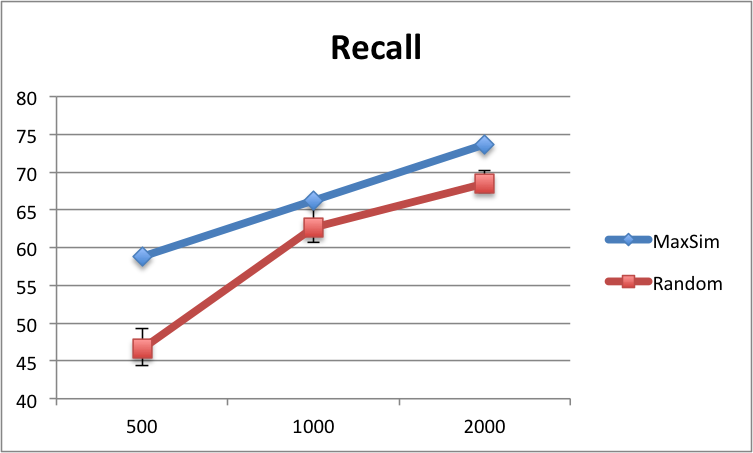
\includegraphics[width=\textwidth]{label_recall.png}
    \caption{Recall}
  \end{subfigure}
  \hspace{2em}
  \begin{subfigure}{0.4\textwidth}
  	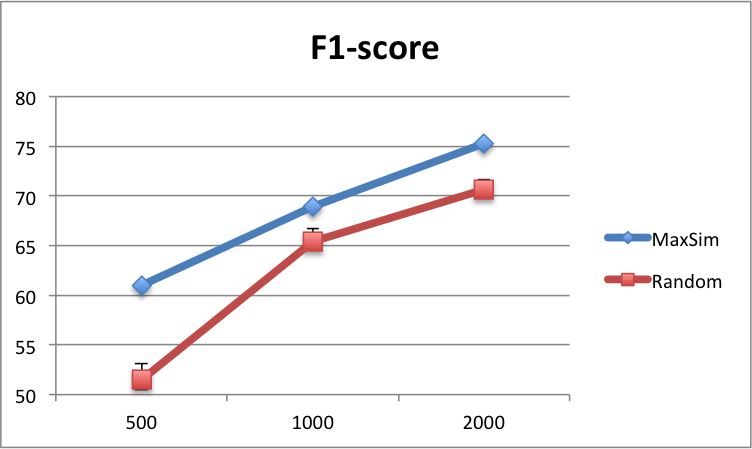
\includegraphics[width=\textwidth]{label_f1.png}
  	\caption{F1-score}
  \end{subfigure}
  \caption{实验结果}
  \label{fig:testing_vs_random}
\end{figure}
从图\ref{fig:testing_vs_random}中可以看出,我们提出了训练集选取方案,在Recall和Precision方面,都稳定的高于随机随机抽样,尤其是在标注量较小时,MaxSim选取的标注集在Recall方面的优势更加明显。

同时我们测试了其他分类模型在两种标注集选取方法下的性能。

可以看出除了KNN以外,SVM,随机森林等分类器在MaxSim上的性能都超过了随机方法。同时,SVM和KNN的总体表现(F1-score)上相差不多,Precision较高而Recall较低,在实际系统中,我们希望提供更加精确的结果,因此,我们最终采用SVM作为分类模型。

\section{错误分析和性能优化}
我对分类错误的样本

\section{本章小结}

